\documentclass[11pt,aspectratio=169]{beamer}

% 直接复用现有主题配置。
% 通用宏包集中在此处；课程内容文件中通常不应再加载宏包。
\usepackage{iftex}
\ifPDFTeX
  \usepackage[T1]{fontenc}
  \usepackage[utf8]{inputenc}
  \usepackage{lmodern}
\else
  \usepackage{fontspec}
  \defaultfontfeatures{Ligatures=TeX}
\fi

\usepackage{amsmath,amssymb,mathtools}
\usepackage{booktabs}
\usepackage{graphicx}
\usepackage{tikz}
\usetikzlibrary{arrows.meta,positioning,shapes.geometric}
\usepackage[most]{tcolorbox}
\usepackage{listings}
\usepackage{xparse}
\usepackage{appendixnumberbeamer}
\usepackage[backend=biber,style=authoryear,maxcitenames=2]{biblatex}
% 修改整套课件配色时，只需要编辑本文件。
\definecolor{Primary}{HTML}{003B6F}
\definecolor{PrimaryLight}{HTML}{EAF2F8}
\definecolor{Accent}{HTML}{D97706}
\definecolor{AccentLight}{HTML}{FFF4E5}
\definecolor{Background}{HTML}{FFFFFF}
\definecolor{Text}{HTML}{20252B}
\definecolor{MutedText}{HTML}{66717E}
\definecolor{RuleColor}{HTML}{D7DEE5}
\definecolor{Success}{HTML}{237A57}
\definecolor{SuccessLight}{HTML}{EAF6F0}
\definecolor{CodeBackground}{HTML}{F5F7F9}
% 字体语义集中定义，避免在每一页手动设置字号与字重。
\ifPDFTeX
  \usefonttheme{professionalfonts}
\else
  \IfFontExistsTF{TeX Gyre Heros}{
    \setsansfont{TeX Gyre Heros}
  }{
    \setsansfont{Latin Modern Sans}
  }
  % TeX Gyre Cursor 随常见 TeX Live 安装提供，适合作为可移植的代码字体。
  \setmonofont{TeX Gyre Cursor}
\fi

\newcommand{\TitleFont}{\fontsize{25}{30}\selectfont\bfseries}
\newcommand{\SubtitleFont}{\large}
\newcommand{\FrameTitleFont}{\large\bfseries}
\newcommand{\BodyFont}{\normalsize}
\newcommand{\SmallFont}{\small}
\newcommand{\CodeFont}{\ttfamily\small}
% Beamer 外观：白底、蓝色主色、无导航按钮、极简页脚。
\mode<presentation>

\useinnertheme{rectangles}
\usefonttheme{professionalfonts}
\setbeamertemplate{navigation symbols}{}
\setbeamertemplate{headline}{}
\setbeamersize{text margin left=0.75cm,text margin right=0.75cm}

\setbeamercolor{normal text}{fg=Text,bg=Background}
\setbeamercolor{structure}{fg=Primary}
\setbeamercolor{alerted text}{fg=Accent}
\setbeamercolor{frametitle}{fg=Primary,bg=Background}
\setbeamercolor{title}{fg=Primary}
\setbeamercolor{subtitle}{fg=MutedText}
\setbeamercolor{author}{fg=Text}
\setbeamercolor{institute}{fg=MutedText}
\setbeamercolor{date}{fg=MutedText}
\setbeamercolor{itemize item}{fg=Primary}
\setbeamercolor{itemize subitem}{fg=Accent}
\setbeamercolor{section in toc}{fg=Text}
\setbeamercolor{section in toc shaded}{fg=MutedText}

\setbeamerfont{frametitle}{series=\bfseries,size=\large}
\setbeamerfont{title}{series=\bfseries,size=\LARGE}
\setbeamerfont{footline}{size=\scriptsize}

\setbeamertemplate{frametitle}{%
  \vspace{0.18cm}%
  \insertframetitle\par
  \vspace{0.10cm}%
  {\color{RuleColor}\rule{\textwidth}{0.5pt}}%
}

\setbeamertemplate{footline}{%
  \leavevmode
  \hbox{%
    \begin{beamercolorbox}[wd=.78\paperwidth,ht=2.8ex,dp=1.2ex,leftskip=.75cm]{normal text}%
      \color{MutedText}\insertshorttitle\enspace |\enspace\insertshortauthor
    \end{beamercolorbox}%
    \begin{beamercolorbox}[wd=.22\paperwidth,ht=2.8ex,dp=1.2ex,rightskip=.75cm plus1fil]{normal text}%
      \hfill\color{MutedText}\insertframenumber\,/\,\inserttotalframenumber
    \end{beamercolorbox}%
  }
}

\setbeamertemplate{title page}{%
  \vfill
  {\color{Primary}\rule{1.2cm}{3pt}\par}
  \vspace{0.55cm}
  {\TitleFont\color{Primary}\inserttitle\par}
  \vspace{0.18cm}
  {\SubtitleFont\color{MutedText}\insertsubtitle\par}
  \vspace{0.9cm}
  {\BodyFont\insertauthor\par}
  {\SmallFont\color{MutedText}\insertinstitute\par}
  \vspace{0.35cm}
  {\SmallFont\color{MutedText}\insertdate\par}
  \vfill
}

\setbeamertemplate{section page}{%
  \vfill
  {\color{MutedText}\large Chapter \insertsectionnumber\par}
  \vspace{0.25cm}
  {\color{Primary}\rule{1.2cm}{3pt}\par}
  \vspace{0.45cm}
  {\fontsize{27}{32}\selectfont\bfseries\color{Primary}\insertsectionhead\par}
  \vfill
}

\AtBeginSection[]{
  \begin{frame}[plain,noframenumbering]
    \sectionpage
  \end{frame}
}

\mode<all>
% 页面级语义环境。正文优先使用这些环境，而不是直接使用 frame。
\newenvironment{titleframe}
  {\begin{frame}[plain,noframenumbering]\titlepage}
  {\end{frame}}

\newenvironment{outlineframe}[1][Outline]
  {\begin{frame}{#1}\tableofcontents[currentsection,hideothersubsections]}
  {\end{frame}}

\newenvironment{theoryframe}[1]
  {\begin{frame}{#1}}
  {\end{frame}}

\newenvironment{exampleframe}[1]
  {\begin{frame}{#1}}
  {\end{frame}}

\newenvironment{figureframe}[1]
  {\begin{frame}{#1}\centering}
  {\end{frame}}

% fragile 页面必须通过 environment=codeframe 告知 Beamer 外层环境名。
\newenvironment{codeframe}[1]
  {\begin{frame}[fragile,environment=codeframe]{#1}}
  {\end{frame}}

\newenvironment{summaryframe}[1][Summary]
  {\begin{frame}{#1}}
  {\end{frame}}

\newcommand{\figurecaption}[1]{%
  \par\vspace{0.35cm}{\small\color{MutedText}#1\par}%
}
% 内容组件：信息框、强调命令、代码样式与常用数学命令。
\tcbset{
  coursebox/.style={
    enhanced,
    boxrule=0pt,
    leftrule=2.5pt,
    arc=1pt,
    outer arc=1pt,
    left=7pt,right=7pt,top=6pt,bottom=6pt,
    fonttitle=\bfseries,
    before skip=6pt,after skip=6pt
  }
}

\newtcolorbox{definitionbox}[1][Definition]{
  coursebox,title=#1,colback=PrimaryLight,colframe=Primary,coltitle=Primary
}
\newtcolorbox{theorembox}[1][Theorem]{
  coursebox,title=#1,colback=PrimaryLight,colframe=Primary,coltitle=Primary
}
\newtcolorbox{proofbox}[1][Proof idea]{
  coursebox,title=#1,colback=SuccessLight,colframe=Success,coltitle=Success
}
\newtcolorbox{remarkbox}[1][Remark]{
  coursebox,title=#1,colback=CodeBackground,colframe=MutedText,coltitle=Text
}
\newtcolorbox{warningbox}[1][Warning]{
  coursebox,title=#1,colback=AccentLight,colframe=Accent,coltitle=Accent
}
\newtcolorbox{importantbox}[1][Important]{
  coursebox,title=#1,colback=AccentLight,colframe=Accent,coltitle=Accent
}

\newcommand{\keyterm}[1]{\textcolor{Primary}{\textbf{#1}}}
\newcommand{\coursecheck}{\textcolor{Success}{\ensuremath{\checkmark}}}

\lstdefinestyle{coursecode}{
  basicstyle=\CodeFont,
  backgroundcolor=\color{CodeBackground},
  keywordstyle=\color{Primary}\bfseries,
  commentstyle=\color{Success},
  stringstyle=\color{Accent},
  numbers=left,
  numberstyle=\tiny\color{MutedText},
  numbersep=8pt,
  frame=single,
  rulecolor=\color{RuleColor},
  framesep=7pt,
  showstringspaces=false,
  breaklines=true,
  columns=fullflexible,
  keepspaces=true,
  tabsize=2
}
\lstset{style=coursecode}

\newcommand{\R}{\mathbb{R}}
\newcommand{\N}{\mathbb{N}}

\addbibresource{../Causal_Inference_C/Beamer/Reference list/bibliography.bib}
\DeclareMathOperator{\Var}{Var}
\newcommand{\E}{\mathbb{E}}
\newcommand{\Prob}{\mathbb{P}}
\newcommand{\ind}{\mathbf{1}}
\tcbset{coursebox/.append style={colbacktitle=Background}}

% Figures live in time-assets/ next to this file.
% If a figure has not been uploaded yet, a placeholder box is shown instead.
\newcommand{\timefigure}[2]{%
  \IfFileExists{time-assets/#2}%
    {\includegraphics[#1]{time-assets/#2}}%
    {\fcolorbox{RuleColor}{CodeBackground}{\parbox[c][2.4cm][c]{4.5cm}{\centering\footnotesize\color{MutedText}Missing figure\\\texttt{time-assets/#2}}}}%
}

% Automatic transition slide for each subsection:
% large section title above, subsection title below.
\newcommand{\sectionsubsectionframe}{%
  \begin{frame}[plain,noframenumbering]
    \vspace{0.9cm}
    {\fontsize{30}{36}\selectfont\bfseries\color{Text}%
      \insertsectionhead\par}

    \vspace{0.45cm}
    \noindent
    {\color{Accent}\rule{1.2cm}{1.3pt}}%
    {\color{RuleColor}\rule{\dimexpr\textwidth-1.2cm\relax}{0.6pt}}

    \vspace{0.45cm}
    {\fontsize{22}{27}\selectfont\bfseries\color{Text}%
      \insertsubsectionhead\par}
    \vfill
  \end{frame}%
}

\AtBeginSubsection[]{\sectionsubsectionframe}
% 课程信息：以后通常只需要修改这里和正文内容。
\title[Causal Inference]{Causal Inference}
\subtitle{Causal Inference and Time}
\author[Zhaoyi]{Zhaoyi}
%\institute[Your University]{Your University}
\date{\today}

\begin{document}

\begin{titleframe}


\end{titleframe}


% Seven sections do not fit into outlineframe at normal size, so use a compact outline.
\begin{frame}{Outline}
\small
\tableofcontents[hideallsubsections]
\end{frame}


\begin{frame}{Overview}
\begin{itemize}
  \item So far, we have focused on \keyterm{cross-sectional data}, where each unit is observed once.
  \item Observing the same population over time (\keyterm{repeated cross-sectional data}), or the same units over time (\keyterm{panel data}) enables additional identification strategies.
  \item In this part of the course, we will discuss:
  \begin{itemize}
    \item Difference-in-Differences models
    \item Fixed-effects models
    \item Synthetic control methods
  \end{itemize}
  \item As always, we start with the simplest model and build upon it.
\end{itemize}
\end{frame}

\begin{frame}{The Central Challenge of Causal Inference with Time}
\begin{importantbox}[Before--after comparisons]
Outcomes may change over time even without treatment.
\end{importantbox}
\begin{itemize}
  \item A before--after comparison cannot distinguish a treatment effect from other changes occurring over time.
  \item \keyterm{Difference-in-differences} uses a comparison group to account for common time trends.
  \item \keyterm{Synthetic control} constructs a comparison group that closely matches the treated unit before treatment.
\end{itemize}
\end{frame}

\begin{frame}{Literature}
\begin{itemize}
  \item Angrist and Pischke (2009) --- Chapter 5
  \item Wager (2024) --- Chapter 13
  \item Roth et al.\ (2023)
\end{itemize}
\vfill
{\footnotesize\color{MutedText}Slide content adapted from Claudia Noack, \emph{Causal Inference and Time}, Causal Inference, University of Bonn, summer semester 2026.}
\end{frame}


\section{Types of Data}

\begin{frame}{Types of Data}
\small
\begin{columns}[T,onlytextwidth]
\begin{column}{0.485\textwidth}
\begin{definitionbox}[Cross-sectional data]
Many units, one period.\\
{\footnotesize\color{MutedText}Example: annual wages for a representative sample of workers in 2024.}
\end{definitionbox}
\begin{definitionbox}[Time-series data]
One unit, many periods.\\
{\footnotesize\color{MutedText}Example: annual wages of one worker from 2000 to 2024.}
\end{definitionbox}
\end{column}
\begin{column}{0.485\textwidth}
\begin{definitionbox}[Repeated cross-sections]
Different samples from the same population in multiple periods.\\
{\footnotesize\color{MutedText}Example: annual wages from a new representative sample of workers in each year from 2000 to 2024.}
\end{definitionbox}
\begin{definitionbox}[Panel data]
Same units observed in multiple periods.\\
{\footnotesize\color{MutedText}Example: annual wages for the same workers, observed from 2000 to 2024.}
\end{definitionbox}
\end{column}
\end{columns}
\begin{itemize}
  \item This chapter covers several temporal data structures: two-period DiD, multi-period panels, repeated cross-sections, and comparative case studies.
\end{itemize}
\end{frame}


\section{Potential Outcome Framework and Time}

\begin{frame}{General Potential Outcome Framework: Two Periods}
\begin{itemize}
  \item We consider settings with a binary treatment and two time periods ($t=0,1$).
  \item Treatment indicator:
  \[
    D_{it}=
    \begin{cases}
      1, & \text{if unit } i \text{ is treated in period } t,\\
      0, & \text{otherwise.}
    \end{cases}
  \]
  \item Four potential outcomes at time $t$: $Y_{it}(d_0,d_1)$, \quad $d_0,d_1\in\{0,1\}$, where:
  \[
    \begin{array}{ll}
      Y_{it}(0,0) & \text{never treated,}\\
      Y_{it}(1,0) & \text{treated only in period } 0,\\
      Y_{it}(0,1) & \text{treated only in period } 1,\\
      Y_{it}(1,1) & \text{treated in both periods.}
    \end{array}
  \]
  \item For each unit and each period, there are four potential outcomes $\Rightarrow$ too complicated, we will simplify this next.
\end{itemize}
\end{frame}

\begin{frame}{Simplified Potential Outcome Framework: Two Periods}
\begin{itemize}
  \item Each unit is treated at most once, in the post-treatment period $t=1$.
  \item Simplified treatment indicator:
  \[
    D_i=
    \begin{cases}
      1, & \text{if treated at } t=1,\\
      0, & \text{otherwise.}
    \end{cases}
  \]
  \item Two potential outcomes for period $t$:
  \[
    Y_{it}(0)\ \ \text{(if untreated at } t=1\text{)},\qquad
    Y_{it}(1)\ \ \text{(if treated at } t=1\text{)}.
  \]
  \item Observed outcome:
  \[
    Y_{it}=Y_{it}(0)+D_i\bigl(Y_{it}(1)-Y_{it}(0)\bigr).
  \]
\end{itemize}
\end{frame}

\begin{frame}{Treatment Effects: Two Periods}
\begin{definitionbox}[Average Treatment Effect at time $t$]
\[\tau_{\text{ATE},t}=\E[Y_{it}(1)-Y_{it}(0)].\]
\end{definitionbox}
\begin{definitionbox}[Average Treatment Effect on the Treated at time $t$]
\[\tau_{\text{ATET},t}=\E[Y_{it}(1)-Y_{it}(0)\mid D_i=1].\]
\end{definitionbox}
\end{frame}

\begin{frame}{What's Next?}
\begin{itemize}
  \item Next, we'll consider:
  \begin{itemize}
    \item Before--After Designs
    \item Difference-in-Differences Models
    \item Fixed-Effects Models
    \item Synthetic Control Methods
  \end{itemize}
  \item For each, we'll discuss identifying assumptions and interpretation.
\end{itemize}
\end{frame}


\section{Before-After Design}

\begin{frame}{Before-After Design: Setting}
\begin{itemize}
  \item Suppose everyone is untreated at $t=0$ (pre-event) and treated at $t=1$ (post-event).
  \item Example:
  \begin{itemize}
    \item Treatment $D_i$: A minimum-wage increase.
    \item Units $i$: Workers.
    \item Outcome $Y_{it}$: Annual wage of worker $i$ at time $t$.
    \item $t=0$: year before minimum wage increase. $t=1$: year after increase.
  \end{itemize}
\end{itemize}
\end{frame}

\begin{frame}{Parameter of Interest}
Our effect of interest is
\[\tau_{\text{ATE},1}=\E[\,Y_{i1}(1)-Y_{i1}(0)\,].\]
However, we only observe $Y_{i1}$ and $Y_{i0}$, so we can identify only
\[\E[\,Y_{i1}-Y_{i0}\,]=\E[\,Y_{i1}(1)-Y_{i0}(1)\,].\]
Note that
\[
\begin{aligned}
  \tau_{\text{ATE},1}&=\E[\,Y_{i1}(1)-Y_{i1}(0)\,]\\
  &=\E\bigl[Y_{i1}(1)-Y_{i0}(1)\bigr]
    +\E\Bigl[\underbrace{Y_{i0}(1)-Y_{i0}(0)}_{\text{anticipation}}\Bigr]
    +\E\Bigl[\underbrace{Y_{i0}(0)-Y_{i1}(0)}_{\text{trend}}\Bigr].
\end{aligned}
\]
\end{frame}

\begin{frame}{Key Identification Assumptions}
\begin{definitionbox}[No anticipation]
It holds that $Y_{i0}(0)=Y_{i0}(1)$ almost surely.
\end{definitionbox}
In period 0, outcomes are unaffected by whether treatment will be received in period 1.

\begin{definitionbox}[No expected anticipation]
It holds that $\E[Y_{i0}(0)]=\E[Y_{i0}(1)]$.
\end{definitionbox}
Allows for random noise but rules out systematic differences.

\medskip
$\Rightarrow$ We need to impose such an assumption also later.
\end{frame}

\begin{frame}{Key Identification Assumptions}
\begin{definitionbox}[Assumption: Constant Potential Outcomes]
$Y_{i0}(0)=Y_{i1}(0)$.
\end{definitionbox}
No time effects in untreated potential outcomes.

\begin{definitionbox}[Assumption: No Trends]
$\E[Y_{i1}(0)]=\E[Y_{i0}(0)]$.
\end{definitionbox}
Allows for random noise but rules out systematic trends.

\medskip
$\Rightarrow$ We will weaken this assumption later.
\end{frame}

\begin{frame}{Identification Result}
\begin{theorembox}[Proposition: Before-After Design]
Under no anticipation and constant potential outcomes,
\[\tau_{\text{ATE},1}=\E[Y_{i1}-Y_{i0}],\]
The observed mean change is a causal effect.
\end{theorembox}
The assumptions can be weakened to hold only in expectation.
\end{frame}

\begin{frame}{Estimation}
\begin{itemize}
  \item Sample estimator for panel data:
  \[\widehat\tau_{\text{ATE},1}=\frac{1}{n}\sum_{i=1}^n(Y_{i1}-Y_{i0}).\]
  \item Equivalently, estimate the linear model
  \[Y_{it}=\alpha+\beta D_{it}+\epsilon_{it},\qquad D_{it}=\ind[t=1],\]
  where $\beta=\tau_{\text{ATE},1}$.
\end{itemize}
\end{frame}

\begin{frame}{Inference}
\begin{itemize}
  \item With panel data, we can easily prove that
  \[\widehat\tau_{\text{ATE},1}\xrightarrow{p}\tau_{\text{ATE},1}
    \quad\text{and}\quad
    \sqrt{n}\,\bigl(\widehat\tau_{\text{ATE},1}-\tau_{\text{ATE},1}\bigr)\xrightarrow{d}N(0,V).\]
  \item $V$ depends on the data-structure.
  \begin{itemize}
    \item For panel data, account for within-unit dependence, for example by clustering standard errors at the unit level.
  \end{itemize}
\end{itemize}
\end{frame}

\begin{frame}{Extensions}
\begin{itemize}
  \item Extensions to multiple periods require stronger assumptions, such as stability of untreated mean outcomes over the relevant pre- and post-treatment periods.
  \item To account for potential trends, we now move to Difference-in-Differences models.
\end{itemize}
\end{frame}


\section{Difference-in-Differences Models}

\begin{frame}{Canonical DiD --- Notation}
\begin{itemize}
  \item We observe panel or repeated cross-sectional data on $Y_{it}$ for $t=0,1$ and $i=1,\dots,n$.
  \item There are two groups: a treated group and a control group.
  \item \textbf{Treatment timing:} Units with $D_i=1$ are treated in period 1; units with $D_i=0$ are never treated.
  \item \textbf{Potential outcomes:} $Y_{it}(d)$ is the potential outcome of unit $i$ in period $t$ if it receives treatment status $d\in\{0,1\}$ in period 1.
  \item \textbf{Observed outcomes:}
  \[Y_{it}=(1-D_i)Y_{it}(0)+D_iY_{it}(1)\]
\end{itemize}
\end{frame}

\begin{frame}{Assumptions --- No Anticipation}
\begin{definitionbox}[No Anticipation]
$Y_{i0}(0)=Y_{i0}(1)$ almost surely.
\end{definitionbox}
\begin{itemize}
  \item \textbf{Intuition:} The outcome in period 0 is not affected by treatment in period 1.
  \item This assumption is often implicit but crucial for interpreting the DiD estimand as a causal effect in period 1.
  \item It fails if individuals change their behavior in anticipation of treatment.
  \item In this simple canonical model, it would suffice to assume that
  \[\E[Y_{i0}(0)\mid D_i=1]=\E[Y_{i0}(1)\mid D_i=1].\]
\end{itemize}
\end{frame}

\begin{frame}{Assumptions --- Parallel Trends}
\begin{definitionbox}[Parallel Trends]
\[\E[Y_{i1}(0)-Y_{i0}(0)\mid D_i=1]=\E[Y_{i1}(0)-Y_{i0}(0)\mid D_i=0]\]
\end{definitionbox}
\begin{itemize}
  \item In the absence of treatment, the change in potential outcomes would have been the same for both groups.
  \item Groups may differ in levels in both periods 0 and 1.
  \item Only the change in expected outcomes must be equal across groups.
  \item This is a weaker assumption than requiring equal outcome levels over time.
\end{itemize}
\end{frame}

\begin{frame}{Visualizing Parallel Trends}
\centering
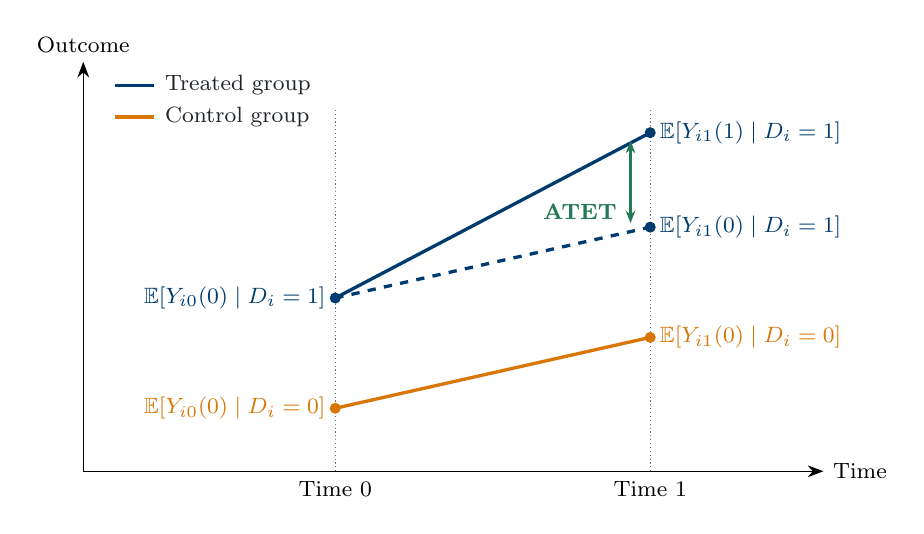
\begin{tikzpicture}[x=1cm,y=1cm,font=\footnotesize]
  % axes
  \draw[-{Stealth[length=2mm]}] (0,0) -- (9.4,0) node[right] {Time};
  \draw[-{Stealth[length=2mm]}] (0,0) -- (0,5.2) node[above] {Outcome};
  % time markers
  \draw[densely dotted,MutedText] (3.2,0) -- (3.2,4.6);
  \draw[densely dotted,MutedText] (7.2,0) -- (7.2,4.6);
  \node[below] at (3.2,0) {Time 0};
  \node[below] at (7.2,0) {Time 1};
  % treated group
  \draw[Primary,very thick] (3.2,2.2) -- (7.2,4.3);
  \fill[Primary] (3.2,2.2) circle (2pt) (7.2,4.3) circle (2pt);
  \node[Primary,left] at (3.2,2.2) {$\E[Y_{i0}(0)\mid D_i=1]$};
  \node[Primary,right] at (7.2,4.3) {$\E[Y_{i1}(1)\mid D_i=1]$};
  % control group
  \draw[Accent,very thick] (3.2,0.8) -- (7.2,1.7);
  \fill[Accent] (3.2,0.8) circle (2pt) (7.2,1.7) circle (2pt);
  \node[Accent,left] at (3.2,0.8) {$\E[Y_{i0}(0)\mid D_i=0]$};
  \node[Accent,right] at (7.2,1.7) {$\E[Y_{i1}(0)\mid D_i=0]$};
  % counterfactual and ATET
  \only<2->{
    \draw[Primary,very thick,dashed] (3.2,2.2) -- (7.2,3.1);
    \fill[Primary] (7.2,3.1) circle (2pt);
    \node[Primary,right] at (7.2,3.1) {$\E[Y_{i1}(0)\mid D_i=1]$};
    \draw[Success,thick,{Stealth[length=1.6mm]}-{Stealth[length=1.6mm]}] (6.95,3.15) -- (6.95,4.2);
    \node[Success,left] at (6.9,3.3) {\textbf{ATET}};
  }
  % legend
  \draw[Primary,very thick] (0.4,4.9) -- (0.9,4.9) node[right,Text] {Treated group};
  \draw[Accent,very thick] (0.4,4.5) -- (0.9,4.5) node[right,Text] {Control group};
\end{tikzpicture}
\end{frame}

\begin{frame}{Potential Violations of the Assumptions}
\begin{itemize}
  \item We will revisit the parallel trends assumption in more detail later.
  \item In practice, treatment assignment may depend on pre-existing differences, which can violate the assumption.
  \item \keyterm{Ashenfelter Dip} (1978):
  \begin{itemize}
    \item Participants in job training programs often experience a drop in earnings just before enrollment.
    \item Due to mean reversion, comparing them to non-participants using DiD can lead to upward-biased estimates.
  \end{itemize}
\end{itemize}
\end{frame}


\subsection{Identification}

\begin{frame}{Identification}
\textbf{Parameter of interest:} The Average Treatment Effect on the Treated (ATET) in period 1:
\[\tau_{\text{ATET}}=\E[Y_{i1}(1)-Y_{i1}(0)\mid D_i=1]\]
\begin{theorembox}[Theorem: Difference-in-Differences Identification]
Under the assumptions of parallel trends and no anticipation, it holds that:
\[
  \tau_{\text{ATET}}=
  \underbrace{\bigl(\E[Y_{i1}\mid D_i=1]-\E[Y_{i0}\mid D_i=1]\bigr)}_{\text{Change in treated group}}
  -\underbrace{\bigl(\E[Y_{i1}\mid D_i=0]-\E[Y_{i0}\mid D_i=0]\bigr)}_{\text{Change in control group}}
\]
\end{theorembox}
This is the canonical ``difference-in-differences'' of population means.
\end{frame}



\subsection{Estimation and Inference}

\begin{frame}{Estimation}
\begin{itemize}
  \item The simplest estimator replaces population means with sample means:
  \[\widehat\tau_{\text{DiD}}=(\bar Y_{11}-\bar Y_{01})-(\bar Y_{10}-\bar Y_{00})\]
  where $\bar Y_{dt}=\frac{1}{n_d}\sum_{i:D_i=d}Y_{it}$ with $n_d=|\{i:D_i=d\}|$.
  \item For panel data, $\widehat\tau_{\text{DiD}}$ is algebraically equivalent to the OLS coefficient $\widehat\beta$ in the \keyterm{two-way fixed effects} model:
  \[Y_{it}=\alpha_i+\phi_t+\beta D_{it}+\varepsilon_{it}\]
  where $D_{it}=D_i\cdot\ind\{t=1\}$.
  \item For panel data, it is also equivalent to $\beta$ in the \keyterm{first-difference} regression:
  \[\Delta Y_i=\alpha+\beta\Delta D_i+u_i\]
\end{itemize}
\end{frame}

\begin{frame}{Asymptotic Distribution in DiD}
\begin{itemize}
  \item Under standard regularity conditions, the estimator $\widehat\tau_{\text{DiD}}$ is approximately normal:
  \[\widehat\tau_{\text{DiD}}\overset{\text{approx}}{\sim}N\bigl(\tau_{\text{ATET}},\sigma^2_{\widehat\tau_{\text{DiD}}}\bigr)\]
  \item Confidence intervals and hypothesis testing are straightforward once a consistent estimator of the variance is available.
  \item Unlike cross-sectional settings, panel data typically exhibit \keyterm{serial correlation} --- e.g., the error term $\varepsilon_{it}$ is often correlated within units.
  \item Standard errors should therefore account for within-unit dependence.
\end{itemize}
\end{frame}

\begin{frame}{Natural Variance Estimator}
For panel data, the natural variance estimator is based on the variance of outcome differences:
\[
  \widehat{\Var}[\widehat\tau_{\text{DiD}}]
  =\frac{\widehat{\Var}(Y_{i1}-Y_{i0}\mid D_i=1)}{n_1}
  +\frac{\widehat{\Var}(Y_{i1}-Y_{i0}\mid D_i=0)}{n_0}.
\]
\begin{itemize}
  \item This variance estimator is robust to within-unit serial correlation.
  \item More generally, inference methods such as the bootstrap or jackknife can be applied by resampling entire units (rows), not individual observations.
\end{itemize}
\end{frame}

\begin{frame}{Concluding Remarks on Canonical DiD}
\begin{itemize}
  \item The DiD design is one of the most widely used tools for estimating causal effects in non-experimental settings.
  \item We will now turn to a classic empirical application of the DiD framework.
  \item Next, we explore fixed effects models, which extend the canonical DiD setup to multiple periods and more general treatment patterns, but require careful interpretation of the underlying parallel-trends assumptions.
  \item In recent years, there has been a surge of econometric research on DiD, introducing new methods, assumptions, and estimands.
  \item We will highlight several strands of this literature, each relaxing different components of the canonical model while preserving others.
\end{itemize}
\end{frame}


\subsection{Case Study: Card and Krueger (1994)}

\begin{frame}{David Card}
\begin{columns}[c,onlytextwidth]
\begin{column}{0.62\textwidth}
\begin{itemize}
  \item Canadian applied Microeconomist.
  \item Key contributions in the field of:
  \begin{itemize}
    \item wage determination, education, inequality, immigration.
  \end{itemize}
  \item Universities: University of California, Berkeley, Princeton University, University of Chicago.
  \item Nobel Prize: 2021.
\end{itemize}
\end{column}
\begin{column}{0.34\textwidth}
\centering
\timefigure{width=\linewidth,height=4.6cm,keepaspectratio}{david-card.png}
\par\medskip{\footnotesize David Card (born 1956)}
\end{column}
\end{columns}
\end{frame}

\begin{frame}{Card and Krueger (1994)}
\small
\begin{itemize}
  \item \textbf{Economic theory prediction:} In a competitive labor market, increasing the minimum wage should reduce employment among minimum wage workers.
  \item But what about the real world?
  \begin{itemize}
    \item \textbf{Ideal experiment:} Randomly assign labor markets to a control group (no change) and a treatment group (minimum wage increase), then compare outcomes.
    \item In reality, policy changes affecting some areas but not others create \keyterm{natural experiments}, though assignment is not random.
  \end{itemize}
  \item Card and Krueger (1994) examine the effect of a minimum wage increase in New Jersey using a Difference-in-Differences (DiD) design.
  \begin{itemize}
    \item In February 1992, New Jersey increased its minimum wage from \$4.25 to \$5.05, while Pennsylvania kept it at \$4.25.
    \item They surveyed approximately 400 fast food restaurants in NJ and PA both before and after the policy change.
  \end{itemize}
\end{itemize}
\end{frame}

\begin{frame}{Distributions of Hourly Wages}
\begin{columns}[T,onlytextwidth]
\begin{column}{0.48\textwidth}
\centering
Before the minimum wage increase in New Jersey (Black)\par\medskip
\timefigure{width=\linewidth,height=5.2cm,keepaspectratio}{wages-before.png}
\end{column}
\begin{column}{0.48\textwidth}
\centering
After the minimum wage increase in New Jersey (Black)\par\medskip
\timefigure{width=\linewidth,height=5.2cm,keepaspectratio}{wages-after.png}
\end{column}
\end{columns}
\end{frame}

\begin{frame}{Example: Card and Krueger (AER, 1994) --- Minimum Wage}
\begin{itemize}
  \item \textbf{Estimation strategy:} Difference-in-Differences method.
  \item \textbf{Results:} Difference in means between New Jersey and Pennsylvania:
\end{itemize}
\begin{center}
{\small\textbf{Table 1:} Simple DiD using sample averages on full-time employment}\par\medskip
\small
\begin{tabular}{lccc}
\toprule
\textbf{Dependent Variable} & \textbf{PA} & \textbf{NJ} & \textbf{NJ -- PA}\\
\midrule
FTE before         & 23.33  & 20.44  & $-2.89$ \\
                   & (1.35) & (0.51) & (1.44) \\
FTE after          & 21.17  & 21.03  & $-0.14$ \\
                   & (0.94) & (0.52) & (1.07) \\
Change in mean FTE & $-2.16$ & 0.59  & 2.76 \\
                   & (1.25) & (0.54) & (1.36) \\
\bottomrule
\end{tabular}
\end{center}
\end{frame}

\begin{frame}{Main Results}
\begin{itemize}
  \item The minimum wage increase did not reduce employment in NJ fast food restaurants compared to those in eastern PA.
  \item Employment actually increased in NJ relative to PA after the policy change.
  \item Wages for low-wage workers increased in NJ relative to PA.
  \item The simple DiD estimate implies a relative increase of about 2.8 full-time-equivalent workers per restaurant in New Jersey.
  \item This finding is evidence against a large immediate employment loss in this particular setting, but it relies on Pennsylvania being a valid comparison group.
\end{itemize}
\end{frame}

\begin{frame}{The Data Debate: Neumark and Wascher (2000)}
\small
\begin{itemize}
  \item The main critique concerned measurement and sample selection, not simply the number of restaurants.
  \item Neumark and Wascher (2000) re-estimated the effect using payroll records for a different sample of restaurants.
  \item Their estimates suggested that employment in New Jersey fell relative to Pennsylvania after the minimum-wage increase.
  \item The disagreement therefore illustrates an important lesson:
\end{itemize}
\begin{importantbox}[Lesson]
A DiD design is only as credible as its outcome measurement, comparison group, and identifying assumptions.
\end{importantbox}
\begin{itemize}
  \item A short before--after comparison also cannot establish whether the New Jersey and Pennsylvania restaurants would have followed parallel trends in the absence of the policy.
\end{itemize}
\end{frame}

\begin{frame}{Card and Krueger's Reply: What Can We Conclude?}
\small
\begin{itemize}
  \item Card et al.\ (2000) argued that the payroll sample used by Neumark and Wascher was not representative.
  \item Using administrative BLS payroll data, Card and Krueger again found similar or slightly faster employment growth in New Jersey than in eastern Pennsylvania.
  \item The evidence from this episode is therefore contested: different data sources and samples led to different conclusions.
  \item The original design provides evidence against an immediate, large negative employment effect of this particular minimum-wage increase on the sampled fast-food restaurants.
  \item It does not establish that minimum-wage increases never reduce employment in other places, industries, time horizons, or policy settings.
\end{itemize}
\end{frame}


\section{Multiple Time Periods}

\begin{frame}{Empirical Settings Are Often More Complicated}
\begin{itemize}
  \item Remember that in the canonical DiD model we had:
  \begin{itemize}
    \item Two periods and a common treatment date.
    \item Identification from parallel trends and no anticipation.
    \item A sufficiently large number of independent sampling units or clusters for reliable inference.
  \end{itemize}
  \item However, in many settings, we have:
  \begin{itemize}
    \item several time periods.
    \item units do not receive the treatment at the same date.
  \end{itemize}
\end{itemize}
\textbf{Question:} How can we generalize these ideas?
\end{frame}

\begin{frame}{Two-way Fixed Effects}
\begin{itemize}
  \item Recall: the classical DiD estimator is numerically equivalent to $\widehat\tau$ from the following OLS regression:
  \[Y_{it}=\alpha_i+\phi_t+\tau D_{it}+\varepsilon_{it}\]
  \begin{itemize}
    \item $\alpha_i$: unit (individual/state/etc.) fixed effect
    \item $\phi_t$: time fixed effect
    \item $D_{it}$: treatment indicator
    \item $\tau$: coefficient of interest
  \end{itemize}
  \item This specification controls for additive unit fixed effects and additive time effects, but does not by itself rule out time-varying confounding or differential trends.
\end{itemize}
\end{frame}

\begin{frame}{Two-way Fixed Effects}
\begin{itemize}
  \item From a statistical perspective, the TWFE model has several advantages:
  \begin{itemize}
    \item It can accommodate multiple time periods.
    \item It flexibly controls for both unit and time fixed effects.
    \item Additional covariates can be easily added linearly.
    \item OLS remains easy to implement.
  \end{itemize}
  \item \textbf{But:} What does $\tau$ actually identify in these settings?
  \item We need to revisit the potential outcomes framework and be careful with interpretation and identification in more complex designs.
\end{itemize}
\end{frame}

\begin{frame}{Treatment Adoption}
\begin{itemize}
  \item With multiple time periods, the number of potential outcomes increases rapidly.
  \item We need to restrict the timing of treatment.
  \item Let $D_{it}$ be a binary treatment indicator that equals one if unit $i$ is treated in period $t$, and zero otherwise.
  \item We maintain the assumption that treatment can only switch from off to on, i.e., $D_{it}\le D_{it'}$ for all $t\le t'$.
  \item We will distinguish between \keyterm{block adoption designs} and \keyterm{staggered adoption designs}.
\end{itemize}
\end{frame}


\subsection{Block Adoption Design}

\begin{frame}{Treatment Adoption}
\begin{definitionbox}[Definition: Block-Adoption Design]
A block adoption design assumes a common treatment start time $H<T$. Units either adopt treatment immediately after $H$ or never adopt. Each unit has an adoption indicator $D_i\in\{0,1\}$ such that
\[D_{it}=D_i\cdot\ind\{t>H\}.\]
\end{definitionbox}
\begin{itemize}
  \item Similarly as before, let $Y_{it}(d)$ denote the potential outcome under the treatment path $D_{is}=d\,\ind\{s>H\}$, where $d\in\{0,1\}$.
\end{itemize}
\end{frame}

\begin{frame}{Key Assumptions for Identification in a Block Design}
\small
\begin{definitionbox}[Assumption: No Anticipation of Treatment]
We assume that potential outcomes do not anticipate treatment. Specifically, we assume that
\[Y_{it}(0)=Y_{it}(1)\quad\text{for } t=1,\dots,H.\]
\end{definitionbox}
Outcomes before treatment do not differ depending on whether a unit is eventually treated.

\begin{definitionbox}[Assumption: Parallel Trends Assumption]
There exist $\beta_2,\dots,\beta_T\in\R$ such that, for all units $i=1,\dots,n$, never-treated potential outcomes satisfy
\[\E\bigl[Y_{it}(0)-Y_{i1}(0)\mid D_i=d\bigr]=\beta_t,\quad t=2,\dots,T\ \text{for } d\in\{0,1\}.\]
\end{definitionbox}
Never-treated potential outcomes evolve the same way on average across groups.
\end{frame}

\begin{frame}{Identification and Estimation in Block Adoption Design}
\begin{itemize}
  \item Consider a block adoption design with several periods before and after the treatment.
  \item Under the above assumptions, based on the usual DiD logic, we can identify
  \[\tau_{\text{ATET},H+1}=\E[Y_{i,H+1}(1)-Y_{i,H+1}(0)\mid D_i=1]\]
  \item A basic DiD uses only two time periods (pre and post), ignoring other available data.
  \[\widehat\tau_{\text{DiD}}=(\bar Y_{1,H+1}-\bar Y_{1,H})-(\bar Y_{0,H+1}-\bar Y_{0,H})\]
  $\Rightarrow$ This ignores useful variation from other time periods.
\end{itemize}
\end{frame}

\begin{frame}{Identification and Estimation in Block Adoption Design}
Using the same logic, we can identify the average treatment effect across all post-periods:
\[\tau_{\text{ATET}}=\frac{1}{T-H}\sum_{t=H+1}^{T}\E[Y_{it}(1)-Y_{it}(0)\mid D_i=1]\]
\begin{itemize}
  \item Average change in outcomes from pre- to post-treatment for treated units minus the same change for controls.
  \item This uses all pre- and post-treatment periods, improving efficiency.
\end{itemize}
\end{frame}

\begin{frame}{Identification and Estimation in Block Adoption Design}
\begin{itemize}
  \item Consider
  \[
  \begin{aligned}
    \widehat\tau_{\text{DiD}}
    &=\frac{1}{n_1}\sum_{i:D_i=1}\left(\frac{1}{T-H}\sum_{t=H+1}^{T}Y_{it}-\frac{1}{H}\sum_{t=1}^{H}Y_{it}\right)\\
    &\quad-\frac{1}{n_0}\sum_{i:D_i=0}\left(\frac{1}{T-H}\sum_{t=H+1}^{T}Y_{it}-\frac{1}{H}\sum_{t=1}^{H}Y_{it}\right).
  \end{aligned}
  \]
  \item This estimator:
  \begin{enumerate}
    \item Uses pre-treatment data to construct a baseline outcome, which is subtracted from post-treatment outcomes.
    \item Compares these post-minus-pre differences between treated and untreated units.
  \end{enumerate}
\end{itemize}
\end{frame}

\begin{frame}{Two-way Fixed-Effects Regression}
\begin{itemize}
  \item In a balanced block-adoption design, the TWFE coefficient coincides with the pooled pre/post DiD estimator.
  \[Y_{it}\sim\alpha_i+\phi_t+\tau D_{it}.\]
  \item This connection is purely algorithmic, and does not rely on well-specification of a linear model.
  \item Mechanistically, we see that the unit fixed effects $\alpha_i$ absorb any additive unit-level baseline effects, and the time fixed effects $\phi_t$ absorb any additive time trends.
\end{itemize}
\end{frame}

\begin{frame}{Generalization of DiD}
\begin{itemize}
  \item When treatment is randomly assigned, $\widehat\tau_{\text{DiD}}$ is unbiased for the ATET.
  \item However, policy adoption decisions are typically endogenous rather than random.
  \item For example:
  \begin{itemize}
    \item Consider a setting where units correspond to the 50 U.S.\ states, and the treatment is a policy adoption decision (e.g., accepting federal subsidies to expand Medicaid).
    \item Then policy adoption is a choice made by states, not the result of random assignment.
  \end{itemize}
\end{itemize}
$\Rightarrow$ We need stronger assumptions or alternative identification strategies.
\end{frame}

\begin{summaryframe}[Summary: Block Adoption Designs]
\begin{itemize}
  \item Units adopt treatment after a shared date $H$ or never.
  \item Identification relies on no anticipation and parallel trends.
  \item This uses all pre- and post-treatment periods and may improve precision when treatment effects are suitably aggregated.
  \item Two-way fixed effects regression recovers the same estimator.
  \item Randomized adoption strengthens identification, but is rare in practice.
\end{itemize}
\end{summaryframe}


\subsection{Staggered Adoption}

\begin{frame}{Treatment Adoption: Staggered Adoption Design}
\begin{definitionbox}[Definition: Staggered-Adoption Design]
Each unit either begins treatment just after a unit-specific event time $1\le H_i\le T-1$, or never receives treatment (in which case we define $H_i=\infty$). Then:
\[D_{it}=\ind\{t>H_i\}.\]
\end{definitionbox}
\begin{itemize}
  \item We define the potential outcome of unit $i$ in period $t$ under treatment timing $h$ as $Y_{it}(h)$.
  \item $Y_{it}(\infty)$ denotes the potential outcome of unit $i$ in period $t$ if it never receives treatment.
\end{itemize}
\end{frame}

\begin{frame}{Assumptions --- Staggered Adoption}
\begin{definitionbox}[No Anticipation of Treatment]
Potential outcomes do not depend on future treatment timing:
\[Y_{it}(h)=Y_{it}(h')\quad\text{for } t\le\min\{h,h'\}.\]
\end{definitionbox}
\begin{definitionbox}[Parallel Trends Assumption]
There exist constants $\beta_2,\dots,\beta_T\in\R$ such that the expected evolution of never-treated potential outcomes is constant across units:
\[\E\bigl[Y_{it}(\infty)-Y_{i1}(\infty)\mid H_i=h\bigr]=\beta_t,\quad t=2,\dots,T,\quad h\in\{1,\dots,T-1,\infty\}.\]
\end{definitionbox}
\end{frame}

\begin{frame}{Why Staggered Adoption Creates Problematic Comparisons}
\footnotesize
\begin{itemize}
  \item Consider three groups:
  \begin{itemize}
    \item Early-treated units adopt in period 2.
    \item Late-treated units adopt in period 3.
    \item Never-treated units are never treated.
  \end{itemize}
  \item Some DiD comparisons are ``clean'':
  \begin{itemize}
    \item Early-treated versus late-treated units before period 3.
    \item Late-treated versus never-treated units after period 3.
  \end{itemize}
  \item But TWFE also compares early-treated and late-treated units after period 3:
  \begin{itemize}
    \item Early-treated units have already been exposed to treatment for longer.
    \item Late-treated units are now treated as well.
    \item Thus, the comparison does not isolate the effect of treatment relative to an untreated counterfactual.
  \end{itemize}
\end{itemize}
\begin{warningbox}[Forbidden comparisons]
Already-treated units can implicitly serve as controls for later-treated units.
\end{warningbox}
\end{frame}

\begin{frame}{What Does TWFE Estimate under Staggered Adoption?}
\small
\begin{itemize}
  \item Define the \keyterm{cohort-time treatment effect}
  \[ATT(h,t)=\E\bigl[Y_{it}(h)-Y_{it}(\infty)\mid H_i=h\bigr],\qquad t>h.\]
  \item A meaningful target parameter must specify how these effects are aggregated:
  \[\theta=\sum_h\sum_{t>h}\omega_{ht}ATT(h,t),\qquad\omega_{ht}\ge0,\qquad\sum_h\sum_{t>h}\omega_{ht}=1.\]
  \item Under no anticipation and parallel trends, the population TWFE coefficient can be written as
  \[\tau^{\text{TWFE}}=\sum_h\sum_{t>h}\omega^{\text{TWFE}}_{ht}ATT(h,t).\]
  \item The weights $\omega^{\text{TWFE}}_{ht}$ depend on the treatment-timing pattern; need not be positive.
  \item Therefore, with treatment-effect heterogeneity across cohorts or event times, $\widehat\tau^{\text{TWFE}}$ need not estimate a transparent average of the treatment effects researchers usually care about.
\end{itemize}
\end{frame}

\begin{frame}{New Estimators (and Estimands!)}
\begin{itemize}
  \item Several new estimators have been developed to address the limitations of TWFE under staggered adoption.
  \item Two key ideas:
  \begin{enumerate}
    \item Be explicit about the \keyterm{target estimand} --- how should we aggregate treatment effects over time and across units?
    \item Use only \keyterm{``clean comparisons''} --- comparisons that do not involve treated units serving as controls.
  \end{enumerate}
  \item A full treatment is beyond this course, but the next slide gives an (incomplete) list of recent approaches.
\end{itemize}
\end{frame}

\begin{frame}{Examples from the Recent Literature}
\small
\begin{itemize}
  \item \textbf{Callaway and Sant'Anna (2021):} Estimate cohort-time treatment effects and aggregate them transparently. Comparison units can be never treated or not yet treated at the relevant date.
  \item \textbf{Sun and Abraham (2021):} Construct cohort-specific event-time effects and aggregate them, avoiding comparisons in which already-treated units act as controls for later-treated units.
  \item \textbf{Borusyak et al.\ (2024) and Gardner (2022):} Estimate the untreated outcome process using observations with $D_{it}=0$, then impute untreated potential outcomes for treated observations.
  \item \textbf{Wooldridge (2023):} Develop regression-based DiD estimators under an index version of parallel trends, allowing for staggered treatment timing and covariates.
  \item These approaches differ in their comparison groups, identifying assumptions, aggregation rules, and inference procedures.
\end{itemize}
\end{frame}

\begin{summaryframe}[Summary: Staggered Adoption and TWFE]
\begin{itemize}
  \item Staggered adoption poses serious challenges for causal identification with TWFE regressions.
  \item TWFE can produce misleading estimates due to negative weighting and contaminated comparisons.
  \item Recent methods focus on clean identification and more interpretable estimands.
\end{itemize}
\begin{importantbox}[Always ask]
What is my estimand? Are my comparisons valid?
\end{importantbox}
\end{summaryframe}


\section{Extensions with Multiple Time Periods}

\begin{frame}{Overview of Extensions under Multiple Time Periods}
\begin{itemize}
  \item We will discuss how to construct event study plots.
  \item We will discuss the parallel trends assumption in more detail:
  \begin{itemize}
    \item Which alternative estimators are available under conditional parallel trends?
    \item How can we assess the plausibility of the parallel-trends assumption?
    \item When does the parallel-trends assumption hold after a monotone transformation of the outcome?
  \end{itemize}
\end{itemize}
\end{frame}


\subsection{Event Study Plot}

\begin{frame}{Treatment Effect Dynamics with Two Groups}
\begin{itemize}
  \item If repeated cross-sections or panel data around the window of treatment are available, DiD can be extended to study dynamic effects over time.
  \item We can then answer questions like:
  \begin{enumerate}
    \item Does treatment effect evolve over time?
    \item Are the assumptions of DiD supported by the data? For instance, do we observe differential pre-treatment changes between future treated and control units?
  \end{enumerate}
\end{itemize}
\end{frame}

\begin{frame}{Treatment Effect Dynamics in a Two-Group Event-Study}
\small
\begin{itemize}
  \item \textbf{Setup:} Panel data under a block-adoption design, with treatment occurring at $t=0$.
  \item \textbf{Regression specification:}
  \[Y_{it}=\phi_i+\lambda_t+\sum_{\tau\neq-1}\gamma_\tau D_i\,\ind\{t=\tau\}+\varepsilon_{it}.\]
  \begin{itemize}
    \item $Y_{it}$: outcome for unit $i$ at time $t$ and $D_i$: treatment indicator ($=1$ if unit $i$ is treated).
    \item $\phi_i$ unit fixed effect and $\lambda_t$ time fixed effect.
    \item For $\tau\ge0$, $\gamma_\tau$ estimates the treatment effect at event time $\tau$. For $\tau<0$, it measures differential pre-treatment changes relative to period $-1$.
  \end{itemize}
  \item Each $\gamma_\tau$ is a DiD estimate comparing the change from period $t=-1$ to $\tau$ between treated and control units:
  \[\gamma_\tau=\bigl(\E[Y_{i\tau}\mid D_i=1]-\E[Y_{i,-1}\mid D_i=1]\bigr)-\bigl(\E[Y_{i\tau}\mid D_i=0]-\E[Y_{i,-1}\mid D_i=0]\bigr).\]
\end{itemize}
\end{frame}

\begin{frame}{Event Study Plot}
\footnotesize
\begin{columns}[c,onlytextwidth]
\begin{column}{0.46\textwidth}
\begin{itemize}
  \item Normalize event time so that $t=0$ corresponds to first treatment period.
  \item Points show effects at each event time.
  \item Confidence intervals capture estimation uncertainty.
\end{itemize}
\end{column}
\begin{column}{0.52\textwidth}
\centering
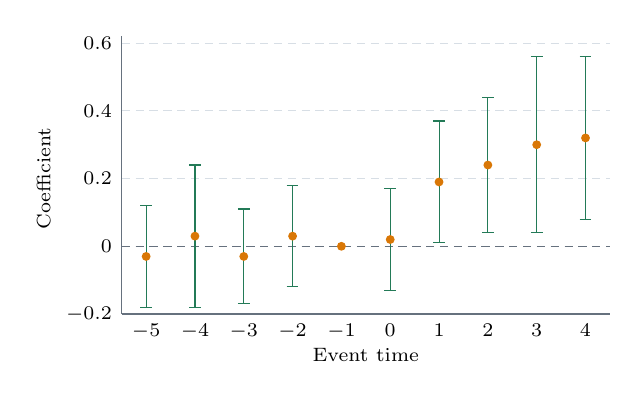
\begin{tikzpicture}[x=0.62cm,y=4.3cm,font=\scriptsize]
  % grid and axes
  \foreach \y in {-0.2,0,0.2,0.4,0.6}{
    \draw[RuleColor,densely dashed] (-5.5,\y) -- (4.5,\y);
    \node[left] at (-5.5,\y) {\pgfmathprintnumber{\y}};
  }
  \draw[MutedText] (-5.5,-0.2) -- (-5.5,0.62);
  \draw[MutedText] (-5.5,-0.2) -- (4.5,-0.2);
  \draw[MutedText,densely dashed] (-5.5,0) -- (4.5,0);
  \foreach \x in {-5,...,4}{
    \node[below] at (\x,-0.2) {$\x$};
  }
  \node[below=9pt] at (-0.5,-0.2) {Event time};
  \node[rotate=90] at (-7.1,0.2) {Coefficient};
  % confidence intervals and point estimates
  \foreach \x/\est/\lo/\hi in {-5/-0.03/-0.18/0.12, -4/0.03/-0.18/0.24, -3/-0.03/-0.17/0.11, -2/0.03/-0.12/0.18, 0/0.02/-0.13/0.17, 1/0.19/0.01/0.37, 2/0.24/0.04/0.44, 3/0.30/0.04/0.56, 4/0.32/0.08/0.56}{
    \draw[Success] (\x,\lo) -- (\x,\hi);
    \draw[Success] (\x-0.12,\lo) -- (\x+0.12,\lo);
    \draw[Success] (\x-0.12,\hi) -- (\x+0.12,\hi);
    \fill[Accent] (\x,\est) circle (1.6pt);
  }
  \fill[Accent] (-1,0) circle (1.6pt);
\end{tikzpicture}
\end{column}
\end{columns}
\begin{itemize}
  \item Focus is on the full trajectory of effects (pre and post), not just a single DiD estimate.
  \begin{itemize}
    \item Testing many periods introduces multiple comparisons.
    \item Pointwise confidence intervals describe uncertainty at individual event times.
    \item Uniform confidence bands are appropriate when interpreting several event-time coefficients jointly.
  \end{itemize}
  \item What would this plot look like if the parallel trends assumption were violated?
\end{itemize}
\end{frame}


\subsection{Placebo Tests}

\begin{frame}{Placebo Outcomes: A Credibility Check}
\small
\begin{itemize}
  \item A \keyterm{placebo outcome} is an outcome that should be unaffected by the treatment, but exposed to similar confounding factors as the main outcome.
  \item A credible placebo outcome requires a substantive argument that the treatment has no relevant direct or indirect effect on it.
  \item Example:
  \begin{itemize}
    \item High-wage employment may be less directly affected by a minimum-wage increase.
    \item However, it is not automatically a valid placebo: substitution across workers, changes in product demand, or price adjustments may also affect high-wage employment.
  \end{itemize}
  \item Interpretation:
  \begin{itemize}
    \item A placebo DiD estimate close to zero is consistent with the design being credible, but does not prove parallel trends.
    \item A non-zero placebo estimate may indicate confounding, spillovers, or that the placebo outcome was not actually unaffected by treatment.
  \end{itemize}
\end{itemize}
\end{frame}


\subsection{Violation of Parallel Trends}

\begin{frame}{Why Might We Be Skeptical of PT?}
\begin{itemize}
  \item Recall PT requires the selection bias to be constant over time.
  \item There are many reasons to be skeptical about this:
  \begin{itemize}
    \item There might be different confounding factors in period 1 as in period 0
    \begin{itemize}
      \item E.g.\ states that pass a minimum wage increase might also change unemployment insurance at the same time
      \item Then UI is a confound in period 1 but not in period 0
    \end{itemize}
    \item The same confounding factors may have different effects on the outcome in different time periods
    \begin{itemize}
      \item Suppose people who enroll in a job training program are more motivated to find a job
      \item Motivation might matter more in a bad economy than in a good economy
    \end{itemize}
  \end{itemize}
\end{itemize}
\end{frame}

\begin{frame}{Violations of Parallel Trends}
\begin{itemize}
  \item \textbf{Conditional Parallel Trends:}
  \begin{itemize}
    \item When overall parallel trends fail, they may hold conditional on covariates $X_i$.
    \item Example: Wage trends differ by education level. If treatment and control groups have different education mixes, parallel trends may hold within each education category.
  \end{itemize}
  \item \textbf{Testing:} Assess violations of (conditional) parallel trends via pre-trend checks, placebo outcomes, and other diagnostics.
\end{itemize}
\end{frame}

\begin{frame}{Conditional Parallel Trends and Overlap}
\begin{itemize}
  \item Let $X_i$ be a vector of time-invariant covariates for unit $i$.
\end{itemize}
\begin{definitionbox}[Conditional Parallel Trends]
\[\E\bigl[Y_{it}(0)-Y_{i0}(0)\mid D_i=1,X_i\bigr]=\E\bigl[Y_{it}(0)-Y_{i0}(0)\mid D_i=0,X_i\bigr]\quad\text{a.s. for } t\ge1.\]
\end{definitionbox}
\begin{itemize}
  \item Conditional parallel trends is neither stronger nor weaker than unconditional parallel trends.
\end{itemize}
\begin{definitionbox}[Overlap]
\[0<\Prob(D_i=1\mid X_i)<1\]
almost surely on the support relevant for treated units.
\end{definitionbox}
\end{frame}

\begin{frame}{Why Additive Covariate Controls Are Not Enough}
\small
\begin{itemize}
  \item In a two-period DiD design, consider the additive regression
  \[Y_{it}=\alpha+\delta D_i+\lambda\ind\{t=1\}+\tau D_i\ind\{t=1\}+X_i^\top\theta+u_{it}.\]
  \item Adding $X_i$ additively allows covariates to affect outcome levels, but imposes that untreated outcome changes do not vary with $X_i$:
  \[\E\bigl[Y_{i1}(0)-Y_{i0}(0)\mid D_i,X_i\bigr]=\lambda.\]
  \item Thus, this regression generally does not accommodate conditional parallel trends.
  \item A more flexible linear specification can allow untreated outcome changes to vary with $X_i$:
  \[
  \begin{aligned}
    Y_{it}={}&\alpha+\delta D_i+\lambda\ind\{t=1\}+\tau D_i\ind\{t=1\}\\
    &+X_i^\top\theta+D_iX_i^\top\rho+\ind\{t=1\}X_i^\top\eta+u_{it}.
  \end{aligned}
  \]
  \item This remains a parametric approach: causal interpretation requires the specified functional form to be correct.
\end{itemize}
\end{frame}

\begin{frame}{Approaches under Conditional Parallel Trends}
\begin{enumerate}
  \item \textbf{Regression models with interactions:} Allow untreated outcome changes to depend on covariates through interactions between $X_i$ and time indicators.
  \item \textbf{Regression adjustment:} Estimate untreated outcome changes among controls conditional on $X_i$, then average predicted changes over the treated covariate distribution.
  \item \textbf{Propensity-score weighting:} Reweight control units so that their covariate distribution resembles that of treated units.
\end{enumerate}
\end{frame}

\begin{frame}{Regression Adjustment under Conditional Parallel Trends}
\begin{itemize}
  \item Consider a two-period panel and define
  \[\Delta Y_i=Y_{i1}-Y_{i0},\qquad m_0(x)=\E[\Delta Y_i\mid D_i=0,X_i=x].\]
  \item Under conditional parallel trends, no anticipation, and overlap,
  \[\tau_{\text{ATET}}=\E[\Delta Y_i\mid D_i=1]-\E[m_0(X_i)\mid D_i=1].\]
  \item Estimation:
  \begin{enumerate}
    \item Estimate $m_0(x)$ using untreated units.
    \item Predict untreated outcome changes for treated units.
    \item Compare observed and predicted changes, averaged over treated units.
  \end{enumerate}
  \item This permits flexible outcome models for $m_0(x)$ and does not require treatment effects to be constant across covariate values.
\end{itemize}
\end{frame}


\subsection{Parallel Trends and Functional Form}

\begin{frame}{Pre-trends to the Rescue\dots}
\begin{itemize}
  \item When several untreated pre-treatment periods are available, they provide useful diagnostics.
  \item We can test whether the groups were moving in parallel prior to the treatment
  \begin{itemize}
    \item If so, some people argue that the assumption that confounding factors are stable seems more plausible
    \item If not, some people argue that it's relatively implausible that would have magically started moving in parallel after treatment date
  \end{itemize}
  \item Testing for pre-trends provides a natural plausibility check on the parallel trends assumption
\end{itemize}
\end{frame}

\begin{frame}{Pre-tests: Limitations of Parallel Trends Checks}
\begin{itemize}
  \item Testing for pre-existing trends is a natural check of the PT assumption, but it has important limitations (Freyaldenhoven et al., 2019; Roth, 2022).
  \item Parallel pre-treatment trends do not guarantee parallel post-treatment trends:
  \begin{itemize}
    \item Concurrent policy changes (e.g., minimum wage and UI reform) can mask divergent post-treatment dynamics.
    \item Differential exposure to macro shocks (e.g., a recession occurring only post-treatment).
  \end{itemize}
\end{itemize}
\end{frame}

\begin{frame}{Pre-tests: Statistical and Inferential Issues}
\begin{itemize}
  \item \textbf{Low power:} Small non-zero pre-trends may go undetected.
  \item \textbf{Selection bias:} Analyzing only cases with ``insignificant'' pre-tests can bias results.
  \item \textbf{What if the pre-test fails?} Use diagnostic and sensitivity tools as in Roth (2022); Rambachan and Roth (2023).
\end{itemize}
\end{frame}

\begin{frame}{Why Might We Be Skeptical of PT?}
\begin{itemize}
  \item Another reason to be skeptical of parallel trends is that its validity will often be \keyterm{functional form dependent}
  \item Consider an example:
  \begin{itemize}
    \item In period 0, all control units have outcome 10; all treated units have outcome 5.
    \item In period 1, all control units have outcome 15.
    \item If treatment hadn't occurred, would treated units' outcome have increased by 5 also (PT in levels)?
    \item Or would they have increased by 50\% ($\sim$PT in logs)?
  \end{itemize}
\end{itemize}
\end{frame}

\begin{frame}{Parallel Trends and Functional Form}
Roth and Sant'Anna (2023) show that PT will depend on functional form unless:
\begin{itemize}
  \item \textbf{Randomization:} treated and control group have same dist.\ of $Y_{it}(0)$ in each period
  \item \textbf{No time effects:} distribution of $Y_{it}(0)$ doesn't change over time for either group
  \item \textbf{A hybrid:} $\theta$ fraction of the population is as good as randomized; the other $1-\theta$ fraction has no time effects.
\end{itemize}
\begin{warningbox}[Warning]
Absent these conditions, PT will be violated for at least some functional form; often hard to know if we chose the right one!
\end{warningbox}
\end{frame}


\section{Synthetic Controls}

\begin{frame}{Introduction to Synthetic Control Methods}
\begin{itemize}
  \item \keyterm{Synthetic Control Methods} (SC) were introduced by Abadie and Gardeazabal (2003) and developed further in Abadie et al.\ (2010).
  \item SC methods are designed to estimate the effects of aggregate-level interventions.
  \item Many policy interventions occur at the level of large units---such as regions, cities, or countries---where only a small number of treated units are available.
  \item Even in experimental settings, disaggregated (micro-level) interventions may be infeasible due to concerns like fairness, logistics, or interference across units.
\end{itemize}
\end{frame}

\begin{frame}{Introduction to Synthetic Control Methods}
\begin{itemize}
  \item In such contexts, comparing treated units to a single untreated unit may not yield a credible counterfactual.
  \item Instead, a weighted combination of untreated units---called a \keyterm{synthetic control}---can more closely match the pre-treatment characteristics of the treated unit.
  \item The SC is constructed as a weighted average of potential control units, with weights chosen to best reproduce the pre-treatment outcomes and covariates of the treated unit.
\end{itemize}
\end{frame}

\begin{frame}{Setup}
\begin{itemize}
  \item Suppose we observe $J+1$ units over periods $1,2,\dots,T$.
  \item Unit ``one'' is exposed to the intervention during periods $T_0+1,\dots,T$.
  \item The remaining $J$ units form the \keyterm{donor pool} of potential controls.
  \item Let $Y_{it}(0)$ be the outcome for unit $i$ at time $t$ in the absence of intervention.
  \item Let $Y_{it}(1)$ be the outcome for unit $i$ at time $t$ if exposed to the intervention.
  \item We aim to estimate the effect of the intervention on the treated unit,
  \[\tau_{1t}=Y_{1t}(1)-Y_{1t}(0)=Y_{1t}-Y_{1t}(0)\]
  for $t>T_0$ and $Y_{1t}$ is the outcome for unit one at time $t$.
\end{itemize}
\end{frame}

\begin{frame}{Setup}
\small
\begin{itemize}
  \item Let $W=(w_2,\dots,w_{J+1})^\top$ with $w_j\ge0$ and $w_2+\dots+w_{J+1}=1$. Each value of $W$ represents a potential synthetic control.
  \item Let $X_1$ be a $(k\times1)$ vector of pre-intervention characteristics for the treated unit.
  \item Similarly, let $X_0$ be a $(k\times J)$ matrix which contains the same variables for the unaffected units of the donor pool.
  \item The vector $W^*=(w_2^*,\dots,w_{J+1}^*)^\top$ is chosen s.t.\ $W^*=\arg\min_{W\in\mathcal{W}}\|X_1-X_0W\|_V$, subject to our weight constraints.
  \item Let $Y_{jt}$ be the value of the outcome for unit $j$ at time $t$. For a post-intervention period $t$ (with $t>T_0$) the synthetic control estimator is:
  \[\widehat\tau_{1t}=Y_{1t}-\sum_{j=2}^{J+1}w_j^*Y_{jt}.\]
\end{itemize}
\end{frame}

\begin{frame}{Weighted Squared Error}
\begin{itemize}
  \item Typically,
  \[\|X_1-X_0W\|=\left(\sum_{h=1}^{k}v_h\bigl(X_{h1}-w_2X_{h2}-\dots-w_{J+1}X_{hJ+1}\bigr)^2\right)^{1/2}.\]
  \item The positive constants $v_1,\dots,v_k$ reflect the predictive power of each predictor on $Y_{1t}(0)$.
  \item $v_1,\dots,v_k$ can be chosen via out-of-sample validation.
\end{itemize}
\end{frame}


\subsection{Application}

\begin{frame}{Application: German Reunification --- Research Design}
\textbf{Research question:} What was the effect of German reunification in 1990 on West German GDP per capita?
\begin{itemize}
  \item \textbf{Treated unit:} West Germany.
  \item \textbf{Intervention:} German reunification in 1990.
  \item \textbf{Outcome:} Annual GDP per capita.
  \item \textbf{Donor pool:} 16 comparable OECD countries:
  \begin{itemize}
    \item Australia, Austria, Belgium, Denmark, France, Greece, Italy, Japan, Netherlands, New Zealand, Norway, Portugal, Spain, Switzerland, United Kingdom, United States.
  \end{itemize}
\end{itemize}
\end{frame}

\begin{figureframe}{Application: German Reunification}
\vfill
\timefigure{width=\textwidth,height=0.78\textheight,keepaspectratio}{german-reunification.png}
\vfill
\end{figureframe}

\begin{frame}{Application: German Reunification}
\begin{center}
\begin{tabular}{lccc}
\toprule
 & West Germany & Synthetic West Germany & OECD Sample\\
\midrule
GDP per capita  & 15808.9 & 15802.24 & 13669.4\\
Trade openness  & 56.8    & 56.9     & 59.8\\
Inflation rate  & 2.6     & 3.5      & 7.6\\
Industry share  & 34.5    & 34.5     & 34.0\\
Schooling       & 55.5    & 55.2     & 38.7\\
Investment rate & 27.0    & 27.0     & 25.9\\
\bottomrule
\end{tabular}
\end{center}
{\scriptsize\color{MutedText}Note: First column reports $X_1$, second column reports $X_0W^\star$, and last column reports a simple average for the 16 OECD countries in the donor pool. GDP per capita, inflation rate, and trade openness are averages for 1981--1990. Industry share (of value added) is the average for 1981--1989. Schooling is the average for 1980 and 1985. Investment rate is averaged over 1980--1984.\par}
\end{frame}

\begin{frame}{Application: German Reunification}
\begin{center}
\begin{tabular}{lc@{\qquad}lc}
\toprule
country $j$ & $W_j^*$ & country $j$ & $W_j^*$\\
\midrule
Australia & 0    & Netherlands    & 0.10\\
Austria   & 0.42 & New Zealand    & 0\\
Belgium   & 0    & Norway         & 0\\
Denmark   & 0    & Portugal       & 0\\
France    & 0    & Spain          & 0\\
Greece    & 0    & Switzerland    & 0.11\\
Italy     & 0    & United Kingdom & 0\\
Japan     & 0.16 & United States  & 0.22\\
\bottomrule
\end{tabular}

\medskip
{\small\textbf{Table 2:} Synthetic control weights $W_j^*$ by country $j$.}
\end{center}
\end{frame}


\subsection{Fit and Validity}

\begin{frame}{Factor Model and Bias Bound}
\begin{itemize}
  \item Abadie et al.\ (2010) establish a bias bound under the \keyterm{factor model}:
  \[Y_{it}(0)=\delta_t+\theta_t^\top Z_i+\lambda_t^\top\mu_i+\varepsilon_{it},\]
  where $Z_i$ are observed features, $\mu_i$ are unobserved features, and $\varepsilon_{it}$ is a unit-level transitory shock, modelled as random noise.
  \item Suppose we choose $W^*$ such that:
  \[\sum_{j=2}^{J+1}w_j^*Z_j=Z_1,\quad\sum_{j=2}^{J+1}w_j^*Y_{j1}=Y_{11},\quad\dots,\quad\sum_{j=2}^{J+1}w_j^*Y_{jT_0}=Y_{1T_0}.\]
  \item In practice, these may hold only approximately.
  \item They show that given this model the bias bound is predicated on close fit, and controlled by the ratio between the scale of $\varepsilon_{it}$ and $T_0$.
\end{itemize}
\end{frame}

\begin{frame}{Fit and Validity}
\begin{itemize}
  \item The credibility of a synthetic control depends on how well it fits the trajectory of $Y_{1t}$ before intervention.
  \item No ex-ante guarantees on fit. If poor, synthetic controls should not be used.
  \item There is a risk of overfitting in settings with small $T_0$, large $J$, and large noise.
  \item Restrict donor pool to units similar to the treated unit to reduce biases.
\end{itemize}
\end{frame}


\subsection{Inference}

\begin{frame}{Diagnostics for Synthetic Control Designs}
\begin{itemize}
  \item A close pre-treatment fit is necessary, but does not prove that the post-treatment gap is causal.
  \item Compare the treated unit's post-treatment gap to \keyterm{placebo gaps} obtained by reassigning treatment to donor units.
  \item Placebo units with poor pre-treatment fit should not be treated as equally informative.
  \item A large post-treatment gap is most credible when it is unusual relative to placebo units with similarly good pre-treatment fit.
\end{itemize}
\end{frame}

\begin{frame}{Inference Challenges in Synthetic Control}
\begin{itemize}
  \item Often there is one treated unit and a fixed donor pool rather than a conventional random sample.
  \item Few donor units limit the usefulness of large-sample approximations.
  \item Data-driven weights make textbook regression standard errors unsuitable.
  \item Abadie et al.\ (2010) therefore assess uncertainty through placebo reassignments rather than conventional $t$-tests.
\end{itemize}
\end{frame}

\begin{frame}{Permutation Inference}
\small
\begin{enumerate}
  \item Treat each donor unit $l=2,\dots,J+1$ as if it were treated and re-estimate its synthetic control using donors $\mathcal{D}_l=\{2,\dots,J+1\}\setminus\{l\}$.
  \item With placebo-specific pre-treatment weights $w_k^{*(l)}$, define $\widehat\alpha_{lt}=Y_{lt}-\sum_{k\in\mathcal{D}_l}w_k^{*(l)}Y_{kt}$.
  \item Compare post-/pre-treatment fit:
  \[R_l=\frac{\Bigl[(T-T_0)^{-1}\sum_{t=T_0+1}^{T}\widehat\alpha_{lt}^{\,2}\Bigr]^{1/2}}{\Bigl[T_0^{-1}\sum_{t=1}^{T_0}\widehat\alpha_{lt}^{\,2}\Bigr]^{1/2}}.\]
  \item Compare the treated unit's ratio $R_1$ with placebo ratios:
  \[p_{\text{placebo}}=\frac{1+\sum_{l\in\mathcal{L}}\ind\{R_l\ge R_1\}}{1+|\mathcal{L}|},\]
  where $\mathcal{L}$ contains units with adequate pre-treatment fit.
\end{enumerate}
\end{frame}

\begin{figureframe}{Permutation Inference: Placebo Ratios}
\timefigure{width=\textwidth,height=0.64\textheight,keepaspectratio}{placebo-rmspe-ratios.png}
\figurecaption{The relevant question is whether the treated unit's post/pre-treatment RMSPE ratio is unusually large relative to well-fitted placebo units.}
\end{figureframe}

\begin{frame}{Interpreting Placebo Comparisons}
\begin{itemize}
  \item Placebo evidence is relative to the donor pool and the quality of pre-treatment fit.
  \item Placebo units with poor pre-treatment fit should receive less weight in the comparison.
  \item Conventional significance levels may be uninformative when the donor pool is small.
  \item A placebo ranking has a randomization interpretation only when treatment could plausibly have been reassigned across the relevant units.
  \item Otherwise, placebo exercises are comparative diagnostics rather than automatic $p$-values.
\end{itemize}
\end{frame}


\subsection{Robustness}

\begin{frame}{Robustness Checks}
\small
\begin{itemize}
  \item \textbf{Leave-one-out:} re-estimate after excluding influential donor units.
  \item \textbf{Donor-pool sensitivity:} vary reasonable donor-pool restrictions.
  \item \textbf{Predictor sensitivity:} assess robustness to alternative predictor sets.
  \item \textbf{Backdating:} assign placebo intervention dates before the actual intervention.
\end{itemize}
\begin{columns}[T,onlytextwidth]
\begin{column}{0.48\textwidth}
\centering
\timefigure{width=\linewidth,height=3.9cm,keepaspectratio}{robustness-backdating.png}
\end{column}
\begin{column}{0.48\textwidth}
\centering
\timefigure{width=\linewidth,height=3.9cm,keepaspectratio}{robustness-leave-one-out.png}
\end{column}
\end{columns}
\end{frame}


\subsection{Conclusions}

\begin{frame}{What Convex Weights Do and Do Not Guarantee}
\begin{itemize}
  \item Synthetic control restricts weights to
  \[w_j\ge0,\qquad\sum_{j=2}^{J+1}w_j=1.\]
  \item The synthetic control therefore lies within the \keyterm{convex hull} of the donor pool: it does not extrapolate beyond observed donor units.
  \item This makes donor contributions transparent and avoids reliance on large negative weights.
  \item But convex weights may fit poorly when the treated unit cannot be approximated by available donors.
  \item Weights are chosen using pre-treatment outcomes, but researchers must still justify the donor pool, predictors, and pre-treatment window.
\end{itemize}
\end{frame}

\begin{frame}{Contextual Requirements for SC Methods}
\small
\begin{itemize}
  \item \textbf{Availability of a comparison group:} units that
  \begin{itemize}
    \item do not adopt interventions similar to the one under investigation,
    \item do not experience large idiosyncratic shocks to the outcome of interest, and
    \item share similar characteristics with the affected unit.
  \end{itemize}
  \item \textbf{No anticipation:} the intervention must not be anticipated by the units prior to implementation.
  \item \textbf{Detectability of effects:}
  \begin{itemize}
    \item Small intervention effects may be indistinguishable from other shocks when the outcome variable is highly volatile.
    \item Some interventions require time to generate effects large enough to be quantitatively detected in the data.
  \end{itemize}
\end{itemize}
\end{frame}

\begin{summaryframe}[Conclusion]
\begin{itemize}
  \item Synthetic controls are a convex combination of similar units.
  \item They are constructed to match pre-treatment outcomes and covariates as closely as possible.
  \item Factor models can rationalize synthetic controls.
  \item Placebo comparisons assess whether the treated unit's post-treatment gap is unusual relative to well-fitted donor units.
\end{itemize}
\end{summaryframe}


\begin{frame}{References}
\scriptsize
\begin{itemize}
  \item Abadie, A., Diamond, A., and Hainmueller, J. (2010). Synthetic control methods for comparative case studies: Estimating the effect of California's tobacco control program. \emph{Journal of the American Statistical Association}, 105(490):493--505.
  \item Abadie, A. and Gardeazabal, J. (2003). The economic costs of conflict: A case study of the Basque Country. \emph{American Economic Review}, 93(1):113--132.
  \item Angrist, J. D. and Pischke, J.-S. (2009). \emph{Mostly Harmless Econometrics: An Empiricist's Companion}. Princeton University Press.
  \item Borusyak, K., Jaravel, X., and Spiess, J. (2024). Revisiting event-study designs: robust and efficient estimation. \emph{Review of Economic Studies}, 91(6):3253--3285.
  \item Callaway, B. and Sant'Anna, P. H. (2021). Difference-in-differences with multiple time periods. \emph{Journal of Econometrics}, 225(2):200--230.
  \item Card, D. and Krueger, A. B. (1994). Minimum wages and employment: A case study of the fast-food industry in New Jersey and Pennsylvania. \emph{The American Economic Review}, 84(4):772--793.
  \item Card, D. and Krueger, A. B. (2000). Minimum wages and employment: a case study of the fast-food industry in New Jersey and Pennsylvania: reply. \emph{American Economic Review}, 90(5):1397--1420.
\end{itemize}
\end{frame}

\begin{frame}{References (continued)}
\scriptsize
\begin{itemize}
  \item Freyaldenhoven, S., Hansen, C., and Shapiro, J. M. (2019). Pre-event trends in the panel event-study design. \emph{American Economic Review}, 109(9):3307--3338.
  \item Gardner, J. (2022). Two-stage differences in differences. \emph{arXiv preprint} arXiv:2207.05943.
  \item Rambachan, A. and Roth, J. (2023). A more credible approach to parallel trends. \emph{Review of Economic Studies}, 90(5):2555--2591.
  \item Roth, J. (2022). Pretest with caution: Event-study estimates after testing for parallel trends. \emph{American Economic Review: Insights}, 4(3):305--322.
  \item Roth, J. and Sant'Anna, P. H. (2023). When is parallel trends sensitive to functional form? \emph{Econometrica}, 91(2):737--747.
  \item Roth, J., Sant'Anna, P. H., Bilinski, A., and Poe, J. (2023). What's trending in difference-in-differences? A synthesis of the recent econometrics literature. \emph{Journal of Econometrics}, 235(2):2218--2244.
  \item Sun, L. and Abraham, S. (2021). Estimating dynamic treatment effects in event studies with heterogeneous treatment effects. \emph{Journal of Econometrics}, 225(2):175--199.
  \item Wager, S. (2024). \emph{Causal Inference: A Statistical Learning Approach}.
  \item Wooldridge, J. M. (2023). Simple approaches to nonlinear difference-in-differences with panel data. \emph{The Econometrics Journal}, 26(3):C31--C66.
\end{itemize}
\end{frame}


\end{document}
